\section{Formal Methods and Verification}
%Boken 12.1 sid 309 310
Its almost impossible to write specification in a natural language and not make
room for different interpretations and misunderstandings. Hence \emph{Formal
Methods} are introduced which are based on formal languages, which rules that
are very precise. Describing a system with formal notation gives rise to the
ability of automating test cases for the system since it is precisely defined.
Formal methods can be used everywhere in the development life cycle and not
only when writing specification for the hole system.
\cite[p.272]{COURSEBOOK:safety-critical}.

In the ISO standard ISO~26262, see section \ref{SEC:ISO26262}, also semi-formal
notation are mentioned. Formal notation needs both semantics and syntax well defined but
semi-formal notation needs only the definition of semantics\cite{ISO26262:car}.

''{\bf Verification} is the process of determining whether the output of a
lifecycle phase fulfils the requirements specified by the previous phase''. \\
Formal verification is the verification of a system using formal methods.
The exact meaning of verification is however confusing \cite{thomas_arts}. The
definition may differ in comparison of academic or industrial use. Even in
different phases of the safety life cycle verification is conducted in various
forms \cite[8:9.2]{ISO26262}.

%''{\bf Testing} is the process used to verify or validate a system or its
%components''.

% \subsection{Formal verification}
% %Skriv n�got luddigt
% Formal verification is very hard to achieve for software, due to the state space
% explosion problem. To achieve formal verification, one must visit every state
% that exists, and prove for each of those states, that the code is correct. State
% space explosion occur when a small increase of elements rapidly raises the
% number of combinations to a computational maximum. %% SKRIV OM!!!!!!!!!!!
%                                 %% framf�r allt sista meningen men ocks� binda
%                                 %% ihop med ISO~26262 och "state-space
%                                 %% complexity"

% \subsection{Semi formal verification}
% %Skriv n�got �n mer luddigt
% Semi formal verification covers a smaller state space than formal
% verification.

\section{Industrial Standards}

%\section{Functional Safety}
% Kanske n�got vi vill skriva om? N�ms i metoden

\subsection {IEC~61508 and ISO~26262}
\label{SEC:ISO26262}
IEC 61508 adopts a four level system for categorizing the
severity of hazards, and a six level system for classifying the frequency of a
hazard \cite{COURSEBOOK:safety-critical}. There is also four risk classes which
are given the values 1-4 where 1 corresponds to the most serious accidents and
four to the least serious \cite{COURSEBOOK:safety-critical}. Based on this, IEC
61508 has a four level classification of safety integrity levels called SIL,
ranged from 1, being the least critical, to 4, being the most critical
\cite{COURSEBOOK:safety-critical}\cite{IEC61508}\cite{Advances:IEC61508}. Each
of the safety integrity levels has a criteria of maximum frequency of failures
which a system built on that SIL must satisfy
\cite{COURSEBOOK:safety-critical}. In other words, a SIL is a level of measure
of the reliability of a safety function \cite{Advances:SIL4}.
% The targeted SIL of the safety function that is going to be implemented has a
% determined number of measurements needed to be taken to achieve the
% classification \cite{Advances:IEC61508}.
Due to the fact that the failure of a safety function can lead to a hazardous
event, the safety integrity of a specific safety function must be of such a
level to ensure that the failure frequency is sufficiently low or that the
consequences of the hazardous event are modified to meet a tolerable risk
\cite{Advances:IEC61508}\cite{Advances:SIL4}. To ensure safety, functions with
SIL 4 need to be tested, and documented the most \cite{IEC61508}.

The automotive functional safety standard, ISO~26262, has adopted a similar
system of SIL, namely ASIL, automotive safety integrity levels. As IEC~61508
there are four integrity levels, named A-D, but there are no direct correlation
between the two \cite{TI:safety_critical}.

%G�r skillnad p� verifikation och verifikation. Dvs vilken fas handlar det om?
% Automotive software for safety related systems is required to be designed,
% implemented and verified by the standard ISO~26262, which handles functional
% safety for automotive equipment. For a higher level of integrity ISO~26262
% strongly recommends that semi formal verification of each module should be
% executed \cite[Part 6]{ISO26262}. It also recommends a formal verification, but
% because of the state-space complexity this is hard to achieve.

%% Skriv om integrationstester mot unittester etc, (6-9, 6-10, 6-11 i ISO)

ISO~26262 describes the full development process from concept to production,
with functional safety in mind. For software development, the standard has a
reference model with different phases of the process, see
figure~\ref{FIG:ISO:phases}. Each phase in the reference model is dependent on
the earlier phases. The reference model has the shape of a V, where the left
side contains all development phases, and the right side contains the test
phases. The work flow from this view starts with the phase ``specification of
software safety requirements''. This phase specifies the software requirements
needed to ensure the stability of the system. They are derived from the
system design specification. This is part of the integration between software
and hardware. The second phase is the ``software architectural design''. It
represent the interaction between all software components. The third phase and
the last development phase, in the model is the ``software unit design and
implementation''. This phase contains the implementation of each module. If the
implementation does not meet the wished safety, maybe the software
architectural design or the specification of the software safety requirements
need to be redesigned.

\begin{figure}
  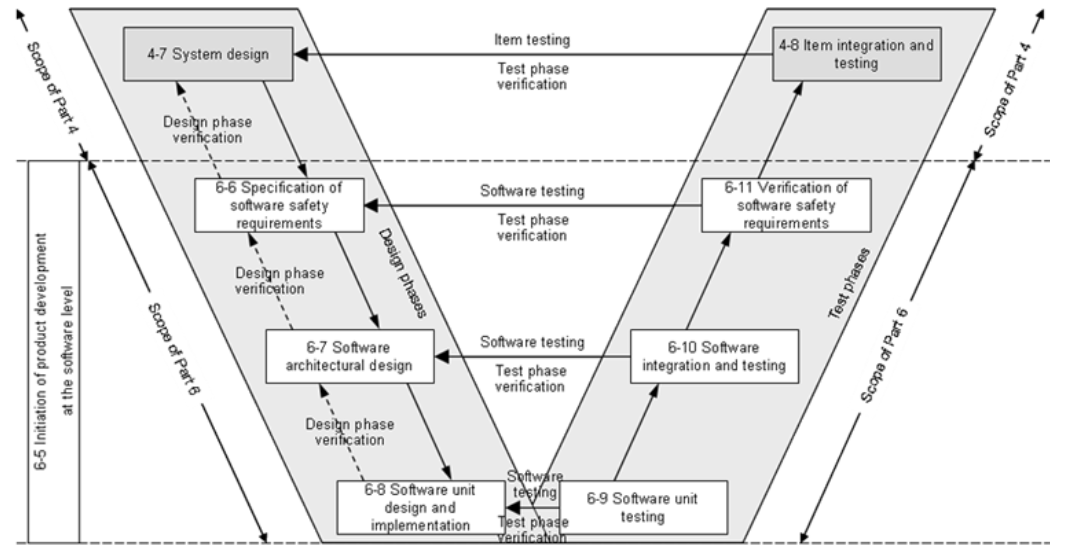
\includegraphics[keepaspectratio, width=\linewidth]{pictures/V}
  \caption{Phases of software development in the standard ISO~26262}
  \label{FIG:ISO:phases}
\end{figure}

Each of these phases is tested thoroughly with the phases ``software unit
testing'', ``software integration and testing'' and ``verification of software
safety requirements''. The unit testing phase tests that the implementation of
the module fulfills the design specifications. If there is failures, one need to
go back to the implementation phase, or if successful go to the phase
integration and testing. This phase objective is to integrate the software units
and demonstrate that the architectural design is correct. A demonstration that
the software safety requirements is fulfilled, is done in the phase
``verification of software safety requirements''.

% ISO~26262 is built on IEC~61508 which is titled Functional Safety of
% Electrical/Electronic/Programmable Electronic Safety-related Systems. IEC~61508
% can be applied to any kind of industry while ISO~26262 is defined only for the
% automotive industry. IEC~61508 have four safety integrity levels (SIL) ranked
% 1-4. SIL 4 is the highest and should be applied where a failure can
% do devastating damage to a large area. %% �r det inte ocks� s� att om det �r
%% ganska farligt men riskerar att h�nda ofta s� ska den ocks� klassas som SIL
%% 4.

\subsection{AUTOSAR (AUTomotive Open System ARchitecture)}
%K�lla http://www.autosar.org/
The AUTOSAR platform has a layered software architecture. This means that the
architecture is divided to a number of different layers, such as the application
layer, runtime environment, the basic software layer, and the
microcontroller. In the figure~\ref{FIG:AUTOSAR:architecture} the basic software
layer is represented as four different parts; services, ECU
abstraction, microcontroller abstraction, and complex drivers.

\begin{figure}[!ht]
  \begin{center}
    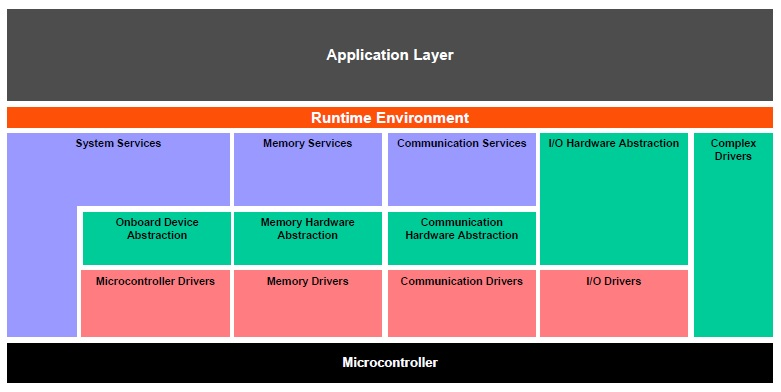
\includegraphics[keepaspectratio, width=\linewidth]{pictures/autosar_architecture.jpg}
  \end{center}
  \caption{The AUTOSAR software architecture. Noticeable is that the basic
    software layer is divided further into three categories with more subsections.}
  \label{FIG:AUTOSAR:architecture}
\end{figure}

The runtime environment is the OS, and the microcontroller is the hardware. The
software running in the application layer is applications such as sensors and
actuators. %% skriva n�got mer om applikationslagret.

%% Saxxat fr�n AUTOSAR Layered software
% Automotive ECUs have the properties: strong interaction with hardware,
% connection to vehicle networks, limited computing power and memory, real time
% system, program execution from internal or external flash memory.

% The AUTOSAR architecture is a generic approach, standard modules can have
% extended functionality and still be compliant.

One example of how the different parts in the basic software layer is
integrated, is the watchdog, which consist of several parts as seen in figure~\ref{FIG:AUTOSAR:watchdog}. The
microcontroller abstraction layer has the drivers for the watchdog, the
interaction with the microcontroller. Then there is the watchdog interface at
the ECU abstraction layer. The watchdog interface is the onboard device
abstraction. Last is the watchdog manager (abbreviated WdgM) which runs as a system service in the
service layer.

\begin{figure}[!ht]
  \begin{center}
    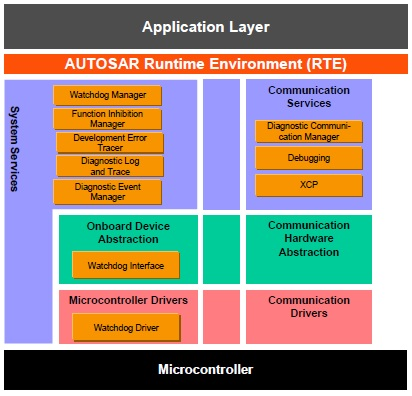
\includegraphics{pictures/watchdog_architecture.jpg}
  \end{center}
  \caption{The Watchdog and some other related modules.}
  \label{FIG:AUTOSAR:watchdog}
\end{figure}

The watchdog have a number of dependencies to other services in the basic
software layer. For example when an error is found by the watchdog, it should be
reported to either the diagnostic event manager or the development error
tracer. Two services used for error management. %% bra eller anus att skriva av
                                %% den ska skicka fel till DEM eller DET n�r vi
                                %% skriver i n�sta avsnitt att det g�r att ta
                                %% bort DEM rapporteringen?

AUTOSAR's concept is to make it possible for vehicle manufacturers to
buy modules from different software developers, which will still work
together in unison. For vehicle manufacturers to have different work
done by the same software developer's module, the standard introduce
configurations. There exist a number of variables to configure. In the
watchdog manager, there is for example variables that specify if the
watchdog manager should report errors to the diagnostic event manager
(DEM), or which type of supervision that should be done and what to supervise.

The current version of AUTOSAR, version 4, has been design with functional
safety in mind. Essential concepts of ISO~26262 have been developed alongside
AUTOSAR.
%% SKRIV MER OM functional safety i version 4 av AUTOSAR


% Some of the specifications in AUTOSAR is left quite open for interpretation.
% %% beskriv varf�r dessa inte �r tillr�ckligt definierade, och varf�r olika
% %% konfigurationer existerar.
% This makes it possible for vehicle developers to have different specifications
% for a configuration. Some parts of those configuration specifications is
% generated into code, while other is manually written or added as a configurable.

\section{Verification Methods}
The standard IEC~61508 propose two methods to say that a program is formal
verified. The key is to model the program into one of the following machines.

\begin{enumerate}
\item \label{enum:FSM} Finite state machines/state transition diagrams
\item Time Petri nets
\end{enumerate}

IEC~61508 emphasises that Time Petri nets are best suited for concurrent
programs. Regarding method \ref{enum:FSM} the following criteria needs to be
satisfied for the implemented state machine to be formal verified:

\begin{description}
\item[completeness] the system must have an action and new state for every input
in every state,
\item[consistency] only one state change is described for each state/input
pair, and
\item[reachability] whether or not it is possible to get from one state to
another by any sequence of inputs.
\end{description}

If the state machine is correctly implemented it exist a correct model of the
%% det �r n�got konstigt med denna meningen men jag kan inte riktigt s�tta
%% fingret p� det.
%% kan vara att: om SM �r korrekt implementerad - s� �r originalprogrammet
%% formellt verifierat. �r detta verkligen allt som kr�vs?
original program, then the original program is formal verified.

Since most program specification are written in natural languages there may be
lots of ambiguities. Consequently a lot of techniques has been developed to reduce
such cases. These techniques are often referred to as semi formal verification,
because they lack of mathematical rigour associated with formal
verification. These methods use textual, graphical or other notation; often
several techniques are used in unity. % These tests may not be

The description of semi formal verification in IEC~61508 states: \\
''Semi-formal methods provide a means of developing a description of a system at
some stage in its development, i.e. specification, design or coding. The
description can in some cases be analysed by machine or animated to display
various aspects of the system behaviour.''


\subsection{QuickCheck}
QuickCheck was invented be Koen Claessen and John Hughes, as a testing module
for Haskell, in 2000.
In 2006 John Hughes founded the Company Quviq together with
Thomas Arts\cite{QUVIQ:about}. Quviq offers a commercial version of QuickCheck for Erlang.
The main difference, except from the programming language, is that
the commercial version of QuickCheck has a C-testing interface. Hence it
possible to test C-code in Erlang with help of QuickCheck. All code for tests
is written in Erlang and checked against API calls to the C-code. It is actually
not necessary to have actual source code; it is enough to only have compiled library
files.

QuickCheck tests a program with specification implemented as properties that
the program must hold \cite{QUICKCHECK:manual}. QuickCheck has guided random
test generation, this means that the samples can be weighted to cover certain
parts of the state-space with more likelihood.
